\documentclass[11pt,a4paper]{article}
\usepackage[utf8]{inputenc}
\usepackage[T1]{fontenc}
\usepackage{lmodern}
\usepackage{amsmath,amssymb,amsthm}
\usepackage{geometry}
\usepackage{booktabs,array,tabularx}
\usepackage{graphicx}
\usepackage{float}
\usepackage{enumitem}
\usepackage[most]{tcolorbox}
\usepackage{hyperref}

\geometry{margin=2.4cm}
\setlength{\parskip}{0.45em}
\setlength{\parindent}{1.2em}

\hypersetup{
    colorlinks=true,
    linkcolor=blue!60!black,
    citecolor=blue!60!black,
    urlcolor=blue!60!black
}

\renewcommand{\abstractname}{Resumo}
\renewcommand{\refname}{Referências Bibliográficas}
\renewcommand{\figurename}{Figura}
\renewcommand{\tablename}{Tabela}
\renewcommand{\contentsname}{Sumário}

\newtheorem{theorem}{Teorema}[section]
\newtheorem{proposition}[theorem]{Proposição}
\newtheorem{corollary}[theorem]{Corolário}
\theoremstyle{definition}
\newtheorem{definition}[theorem]{Definição}
\newtheorem{example}[theorem]{Exemplo}
\theoremstyle{remark}
\newtheorem{remark}[theorem]{Observação}

\newtcolorbox{exambox}[1][]{
    colback=white,
    colframe=black!75,
    boxrule=0.75pt,
    arc=2pt,
    left=8pt,
    right=8pt,
    top=6pt,
    bottom=6pt,
    fonttitle=\bfseries\small,
    coltitle=black,
    colbacktitle=black!8,
    #1
}

\title{\textbf{Quando a Distância até a Média Engana:\\Comparação de Somas de Dados e o Ponto de Virada entre Distribuições}}

\author{
    \textbf{Ítalo Leal}\\
    {\small Curso de Sistemas de Informação}\\
    {\small Departamento de Ciência da Computação (DCC / ICEx)}\\
    {\small Universidade Federal de Minas Gerais (UFMG)}\\
    {\small \texttt{italoleallanasantos@gmail.com}}
}

\date{Novembro de 2026}

\begin{document}

\maketitle

\begin{abstract}
\noindent
Um exercício clássico de probabilidade discreta pergunta se é mais provável obter soma $8$ lançando dois dados ou três dados honestos de seis faces, repetindo a pergunta em seguida para a soma $9$. Em uma avaliação de Matemática Discreta na UFMG, estudantes responderam a ambos os itens sem enumerar as combinações, comparando apenas a distância absoluta entre a soma alvo e o valor esperado de cada lançamento ($E[S_2] = 7$ e $E[S_3] = 10{,}5$). Embora esse raciocínio acerte tanto para a soma $8$ quanto para a soma $9$, ele se apoia na hipótese implícita de que o ponto de virada entre duas distribuições coincide com a média aritmética de suas esperanças. Neste artigo, mostramos que essa heurística falha em duas direções opostas: quando o número de dados cresce de forma espaçada (como em $2$ dados contra $5$ dados na soma $12$), a maior variância desloca o ponto de virada para baixo da média aritmética; já quando comparamos quantidades consecutivas maiores (como $4$ dados contra $5$ dados na soma $16$), a vantagem na altura do pico desloca o ponto de virada para cima da média aritmética. Utilizando a aproximação normal pelo Teorema Central do Limite, demonstramos que a constância da razão entre média e variância em somas de variáveis independentes e identicamente distribuídas elimina o termo linear na equação de log-verossimilhança. Disso resulta uma fórmula fechada para o ponto de interseção contínuo $x^*(n,m)$, governada pela média geométrica das esperanças corrigida pela média logarítmica e pelo coeficiente de variação. Por fim, confrontamos a expressão contínua com a distribuição combinatória exata de De Moivre e explicamos por que o par $(3,5)$ na soma $14$ produz a única interseção discreta exata não trivial para dados de seis faces.

\vspace{0.5em}
\noindent\textbf{Palavras-chave:} probabilidade discreta, soma de dados, teorema central do limite, média geométrica, média logarítmica, fronteira de decisão.
\end{abstract}

\section{Introdução e Origem do Problema}

O estudo das probabilidades associadas à soma de dados honestos acompanha a própria fundação da teoria das probabilidades. No início do século XVII, Galileu Galilei redigiu o ensaio \textit{Sopra le Scoperte dei Dadi} \cite{galilei1620,david1962} para responder a uma dúvida de jogadores florentinos: no lançamento de três dados de seis faces, por que a soma $10$ ocorre com maior frequência do que a soma $9$, se ambos os valores admitem exatamente seis partições inteiras com três parcelas de $1$ a $6$? Galileu resolveu o impasse distinguindo os três dados por ordem de lançamento e mostrando que as seis partições da soma $10$ se desdobram em $27$ trincas ordenadas nas $6^3 = 216$ equiprováveis, ao passo que as seis partições da soma $9$ geram apenas $25$ trincas. Pouco menos de um século depois, Abraham de Moivre generalizou a contagem no tratado \textit{De Mensura Sortis} (1711) e no livro \textit{The Doctrine of Chances} (1718) \cite{demoivre1711,demoivre1718}, obtendo por funções geradoras e inclusão-exclusão a expressão exata para a soma de $n$ dados de $s$ faces.

Nos problemas estudados por Galileu e De Moivre, a quantidade de dados $n$ permanece fixa e comparam-se duas somas distintas $k_1$ e $k_2$. Uma inversão natural dessa pergunta aparece como exercício no livro de Kenneth H. Rosen \cite[Cap.~7, Seção~7.1, Exercícios~36 e~37]{rosen2019} e foi proposta pelo professor Jeroen van de Graaf na primeira prova de Matemática Discreta do Departamento de Ciência da Computação da UFMG: fixada a soma alvo $k$, qual quantidade de dados torna o resultado mais provável?

A Figura~\ref{fig:questao_p1} reproduz a Questão~4 da avaliação (dividida nos itens (a) para a soma $8$ e (b) para a soma $9$), juntamente com a resolução combinatória padrão por listagem das tuplas favoráveis.

\begin{figure}[H]
\centering
\begin{exambox}[title={Questão 4 da Prova de Matemática Discreta (DCC / ICEx / UFMG)}]
\small
\textbf{(a) O que é mais provável: sair um total de 8 quando dois dados são lançados ou sair um total de 8 quando três dados são lançados?}

\vspace{0.25em}
\renewcommand{\arraystretch}{1.18}
\begin{tabularx}{\textwidth}{@{}p{0.37\textwidth}|X@{}}
\textbf{Lançamento de 2 dados} & \textbf{Lançamento de 3 dados} \\
\hline
\textbf{Soma 8} ($5$ pares ordenados): &
\textbf{Soma 8} ($21$ trincas ordenadas): \\
$(2,6),\; (6,2),\; (3,5),$ &
$(1,1,6), (1,6,1), (6,1,1), (1,2,5), (1,5,2), (2,1,5), (2,5,1),$ \\
$(5,3),\; (4,4)$ &
$(5,1,2), (5,2,1), (1,3,4), (1,4,3), (3,1,4), (3,4,1), (4,1,3),$ \\
& $(4,3,1), (2,2,4), (2,4,2), (4,2,2), (2,3,3), (3,2,3), (3,3,2)$ \\[0.25em]
Probabilidade: $\displaystyle P(S_2 = 8) = \frac{5}{36} = \frac{30}{216}$ &
Probabilidade: $\displaystyle P(S_3 = 8) = \frac{21}{216}$
\end{tabularx}
\vspace{0.2em}
\begin{center}
$\displaystyle \boxed{\frac{30}{216}} > \frac{21}{216} \quad \Longrightarrow \quad$ \textbf{Mais provável com 2 dados.}
\end{center}

\hrule
\vspace{0.35em}
\textbf{(b) O que é mais provável: sair um total de 9 quando dois dados são lançados ou sair um total de 9 quando três dados são lançados?}

\vspace{0.2em}
\textbf{2 dados} ($4$ pares): $(3,6),\; (4,5),\; (5,4),\; (6,3) \;\longrightarrow\; \displaystyle P(S_2 = 9) = \frac{4}{36} = \frac{24}{216}$.

\textbf{3 dados} ($25$ trincas, separadas pelo valor do primeiro dado $d_1 \in \{1,\dots,6\}$):
\vspace{-0.4em}
\begin{align*}
d_1 = 1: &\; (1,2,6), (1,3,5), (1,4,4), (1,5,3), (1,6,2) & d_1 = 4: &\; (4,1,4), (4,2,3), (4,3,2), (4,4,1) \\
d_1 = 2: &\; (2,1,6), (2,2,5), (2,3,4), (2,4,3), (2,5,2), (2,6,1) & d_1 = 5: &\; (5,1,3), (5,2,2), (5,3,1) \\
d_1 = 3: &\; (3,1,5), (3,2,4), (3,3,3), (3,4,2), (3,5,1) & d_1 = 6: &\; (6,1,2), (6,2,1)
\end{align*}
\vspace{-0.8em}
\begin{center}
$\displaystyle P(S_3 = 9) = \frac{5+6+5+4+3+2}{216} = \frac{25}{216} > \frac{24}{216} \quad \Longrightarrow \quad \boxed{\textbf{Mais provável com 3 dados.}}$
\end{center}
\end{exambox}
\caption{Reconstrução da Questão 4 da prova de Matemática Discreta e de sua resolução combinatória.}
\label{fig:questao_p1}
\end{figure}

O que motivou o presente trabalho foi a solução alternativa apresentada por um colega de turma naquela avaliação. Em vez de contar os pares e trincas que somam $8$ e $9$, o estudante observou que a média (esperança) de um dado honesto vale $\mu_1 = 3{,}5$, de modo que a soma de dois dados tem média $E[S_2] = 7{,}0$ e a soma de três dados tem média $E[S_3] = 10{,}5$. A partir disso, argumentou que:
\begin{enumerate}[label=(\alph*), topsep=0.2em, itemsep=0.15em]
    \item Para a soma $k = 8$, a distância até a média de dois dados é $|8 - 7{,}0| = 1{,}0$, menor do que a distância até a média de três dados, $|8 - 10{,}5| = 2{,}5$; logo, dois dados seriam mais prováveis.
    \item Para a soma $k = 9$, a distância até a média de três dados cai para $|9 - 10{,}5| = 1{,}5$, menor do que $|9 - 7{,}0| = 2{,}0$; logo, três dados seriam mais prováveis.
\end{enumerate}

Na correção inicial, a resposta não recebeu a pontuação integral porque a justificativa não provava que menor distância à média implicava maior probabilidade. Após revisão e discussão com o professor Jeroen van de Graaf, os pontos foram concedidos pelo raciocínio criativo, mas permaneceu a pergunta matemática de fundo: \textit{por que o critério da distância até a média acertou os dois itens da prova e em que condições ele passa a errar?}

Nas seções seguintes, respondemos a essa questão tanto no domínio combinatório discreto quanto na aproximação contínua. Mostramos que o critério da distância até a média equivale a fixar a fronteira de decisão na média aritmética das esperanças, $\mu_A(n,m) = \frac{1}{2}(\mu_n + \mu_m)$, e provamos que a fronteira assintótica real é dada por uma combinação entre a média geométrica e a média logarítmica.

\section{Distribuição Exata no Domínio Discreto}

Seja $S_n = \sum_{i=1}^n D_i$ a soma dos resultados de $n$ lançamentos independentes de um dado honesto de $s$ faces numeradas de $1$ a $s$ (no caso padrão, $s = 6$). Cada variável $D_i$ segue uma distribuição uniforme discreta em $\{1, 2, \dots, s\}$, com esperança e variância dadas por:
\begin{equation}
\mu_1 = E[D_i] = \frac{s + 1}{2}, \qquad \sigma_1^2 = \text{Var}(D_i) = \frac{s^2 - 1}{12}.
\label{eq:parametros_1d}
\end{equation}
Para $s = 6$, temos $\mu_1 = \frac{7}{2} = 3{,}5$ e $\sigma_1^2 = \frac{35}{12} \approx 2{,}9167$. Pela linearidade da esperança e pela independência entre os lançamentos, a soma $S_n$ possui esperança e variância lineares em $n$:
\begin{equation}
\mu_n = E[S_n] = n\mu_1, \qquad \sigma_n^2 = \text{Var}(S_n) = n\sigma_1^2.
\label{eq:parametros_nd}
\end{equation}

O número de resultados favoráveis $N(n, k, s) = \#\{(d_1,\dots,d_n) \in \{1,\dots,s\}^n : d_1 + \dots + d_n = k\}$ é o coeficiente de $x^k$ no polinômio gerador:
\begin{equation}
P_{n,s}(x) = \left(x + x^2 + \dots + x^s\right)^n = x^n \left(\frac{1 - x^s}{1 - x}\right)^n = x^n (1 - x^s)^n (1 - x)^{-n}.
\end{equation}
Expandindo $(1 - x^s)^n = \sum_{j=0}^n (-1)^j \binom{n}{j} x^{sj}$ e $(1 - x)^{-n} = \sum_{r=0}^\infty \binom{n + r - 1}{n - 1} x^r$, obtém-se a fórmula clássica de De Moivre \cite{demoivre1711,uspensky1937,feller1968}:
\begin{equation}
P(S_n = k) = \frac{N(n, k, s)}{s^n} = \frac{1}{s^n} \sum_{j=0}^{\lfloor \frac{k - n}{s} \rfloor} (-1)^j \binom{n}{j} \binom{k - sj - 1}{n - 1},
\qquad n \le k \le sn.
\label{eq:demoivre}
\end{equation}

Computacionalmente, também é imediato calcular $N(n, k, s)$ por programação dinâmica usando a relação de recorrência $N(n, k, s) = \sum_{f=1}^s N(n-1, k-f, s)$ combinada com a identidade de simetria $N(n, k, s) = N(n, n(s+1) - k, s)$. A Tabela~\ref{tab:distribuicao_1a6} apresenta as probabilidades exatas de soma para $n \in \{1, 2, 3, 4, 5, 6\}$ dados de $6$ faces no intervalo $6 \le k \le 19$, onde ocorrem as transições entre curvas vizinhas.

\begin{table}[H]
\centering
\caption{Probabilidades exatas $P(S_n = k)$ (em porcentagem) para $n = 1, \dots, 6$ dados de $6$ faces no intervalo $6 \le k \le 19$. Em negrito, destaca-se o valor em que $P(S_m = k)$ supera ou iguala $P(S_{m-1} = k)$.}
\label{tab:distribuicao_1a6}
\vspace{0.3em}
\small
\begin{tabular}{@{}ccccccc@{}}
\toprule
\textbf{Soma ($k$)} & \textbf{$P(S_1 = k)$} & \textbf{$P(S_2 = k)$} & \textbf{$P(S_3 = k)$} & \textbf{$P(S_4 = k)$} & \textbf{$P(S_5 = k)$} & \textbf{$P(S_6 = k)$} \\
\midrule
6  & 16,67\% & 13,89\% &  4,63\% &  0,77\% &  0,06\% & 0,002\% \\
7  &  0,00\% & \textbf{16,67\%} &  6,94\% &  1,54\% &  0,19\% & 0,01\%  \\
8  &  0,00\% & 13,89\% &  9,72\% &  2,70\% &  0,45\% & 0,05\%  \\
9  &  0,00\% & 11,11\% & \textbf{11,57\%} &  4,32\% &  0,90\% & 0,12\%  \\
10 &  0,00\% &  8,33\% & 12,50\% &  6,17\% &  1,62\% & 0,27\%  \\
11 &  0,00\% &  5,56\% & 12,50\% &  8,02\% &  2,64\% & 0,54\%  \\
12 &  0,00\% &  2,78\% & 11,57\% &  9,65\% &  3,92\% & 0,98\%  \\
13 &  0,00\% &  0,00\% &  9,72\% & \textbf{10,80\%} &  5,40\% & 1,62\%  \\
14 &  0,00\% &  0,00\% &  6,94\% & 11,27\% &  6,94\% & 2,49\%  \\
15 &  0,00\% &  0,00\% &  4,63\% & 10,80\% &  8,37\% & 3,57\%  \\
16 &  0,00\% &  0,00\% &  2,78\% &  9,65\% &  9,45\% & 4,82\%  \\
17 &  0,00\% &  0,00\% &  1,39\% &  8,02\% & \textbf{10,03\%} & 6,12\%  \\
18 &  0,00\% &  0,00\% &  0,46\% &  6,17\% & 10,03\% & 7,35\%  \\
19 &  0,00\% &  0,00\% &  0,00\% &  4,32\% &  9,45\% & 8,37\%  \\
\bottomrule
\end{tabular}
\end{table}

\subsection{Um Caso Raro no Domínio Discreto: O Empate Exato entre 3 e 5 Dados}

Na etapa inicial desta investigação, quando as probabilidades da Tabela~\ref{tab:distribuicao_1a6} foram tabuladas em planilha eletrônica para buscar pontos em que duas distribuições discretas assumem exatamente o mesmo valor positivo, $P(S_n = k) = P(S_m = k) > 0$, observou-se na linha $k = 14$ uma igualdade exata entre $3$ dados e $5$ dados:
\[
P(S_3 = 14) = \frac{15}{216} = \frac{5}{72} \approx 6{,}944\%,
\qquad
P(S_5 = 14) = \frac{540}{7776} = \frac{15 \times 36}{216 \times 36} = \frac{5}{72} \approx 6{,}944\%.
\]
Como $E[S_3] = 10{,}5$ e $E[S_5] = 17{,}5$, o inteiro $k = 14$ coincide exatamente com a média aritmética das duas esperanças, $\mu_A(3,5) = \frac{10{,}5 + 17{,}5}{2} = 14$. Uma busca exaustiva em todos os pares $1 \le n < m \le 30$ mostra que $(n, m) = (3, 5)$ em $k = 14$ é o \textbf{único} empate não trivial entre duas somas de dados de seis faces nessa faixa. Na Seção~\ref{sec:comparacao_medias}, veremos que esse empate não decorre de uma propriedade geral da média aritmética, mas do fato de que, especificamente para o par $(3,5)$, o ponto de interseção contínuo vale $x^*(3,5) \approx 13{,}9615$, quase coincidindo com o inteiro $14$.

\section{Por que a Heurística da Distância até a Média Falha}
\label{sec:falacia}

Formalizemos o raciocínio utilizado na prova. Dados dois números de dados $n < m$ e uma soma alvo $k$, a heurística da distância até a média decide em favor de $n$ dados quando $|k - \mu_n| < |k - \mu_m|$, e em favor de $m$ dados quando $|k - \mu_m| < |k - \mu_n|$. Como $\mu_n < \mu_m$, a equação $|x - \mu_n| = |x - \mu_m|$ tem solução única na média aritmética das esperanças:
\begin{equation}
\mu_A(n, m) = \frac{\mu_n + \mu_m}{2} = \mu_1 \left(\frac{n + m}{2}\right).
\label{eq:media_aritmetica}
\end{equation}
Portanto, usar a distância até a média como critério equivale a supor que as duas curvas de probabilidade se cruzam exatamente no ponto médio $\mu_A(n,m)$.

Essa suposição ignora duas propriedades fundamentais da soma de variáveis independentes (ilustradas na Figura~\ref{fig:distribuicoes_1a6}):
\begin{enumerate}[topsep=0.2em, itemsep=0.2em]
    \item \textbf{Alargamento da dispersão:} A variância $\sigma_n^2 = n\sigma_1^2$ cresce linearmente com o número de dados, e o desvio padrão $\sigma_n = \sigma_1 \sqrt{n}$ cresce com $\sqrt{n}$. A distribuição de $m$ dados espalha sua massa por um intervalo muito mais amplo do que a de $n$ dados.
    \item \textbf{Queda da altura máxima:} Como a soma total das probabilidades é sempre igual a $1$ e o desvio padrão cresce com $\sqrt{n}$, a probabilidade máxima no centro da distribuição cai na proporção de $1/\sqrt{n}$. Por exemplo, $\max_k P(S_2 = k) = P(S_2 = 7) = 16{,}67\%$, enquanto $\max_k P(S_6 = k) = P(S_6 = 21) \approx 9{,}28\%$.
\end{enumerate}

\begin{figure}[H]
\centering
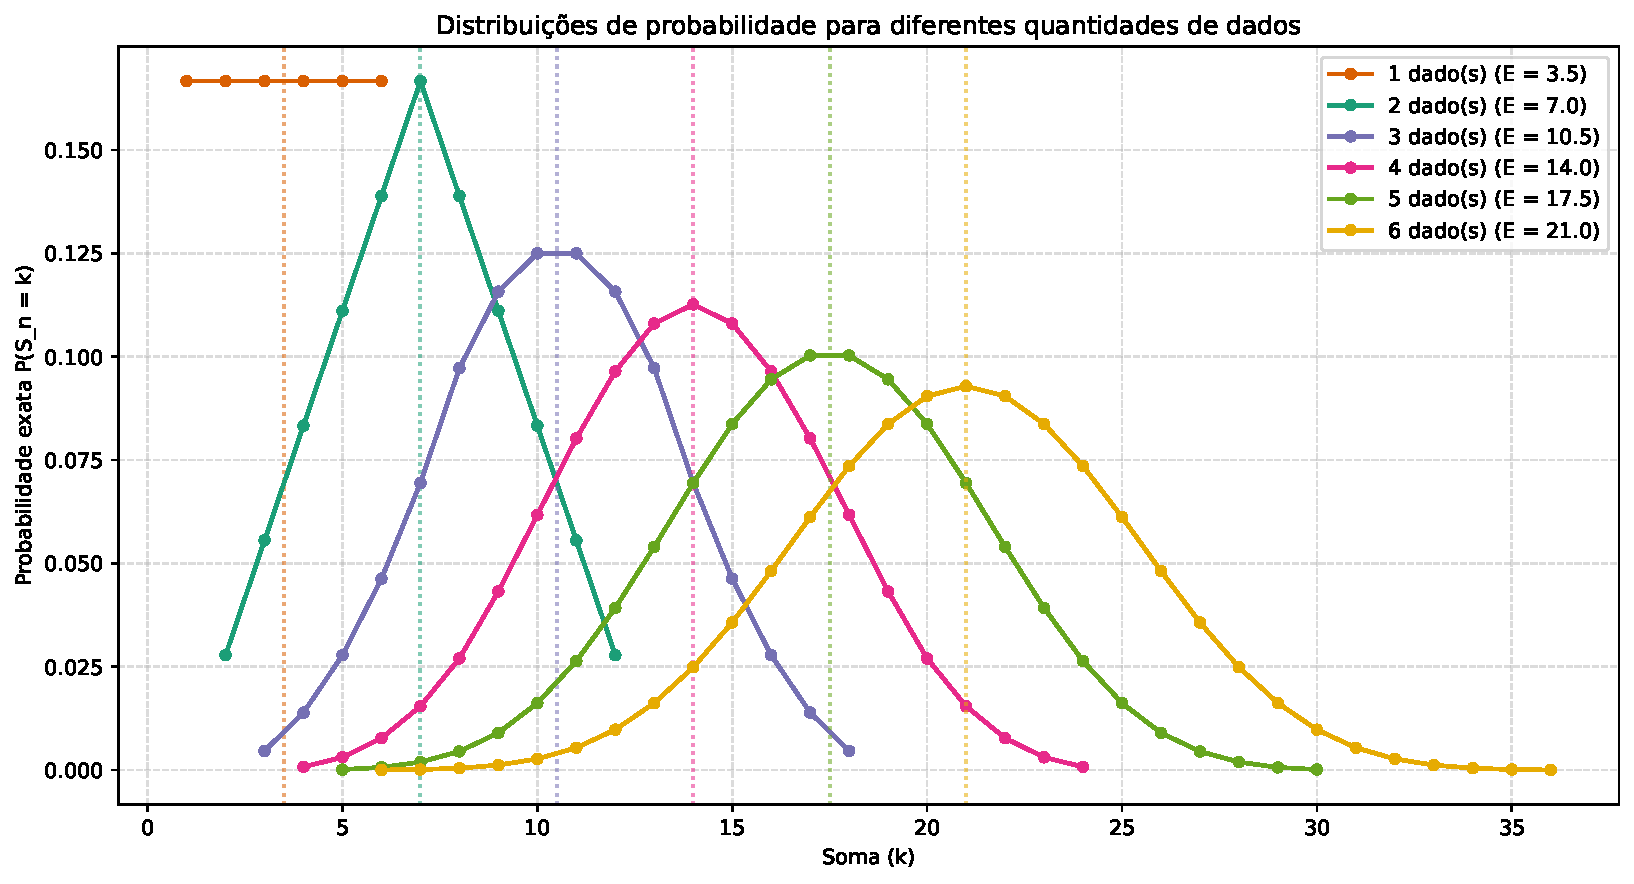
\includegraphics[width=0.88\textwidth]{figures/distribuicoes_1d_a_6d.pdf}
\caption{Distribuições exatas de probabilidade para $1$ a $6$ dados de seis faces. As linhas verticais pontilhadas indicam as esperanças $\mu_n = 3{,}5n$. À medida que $n$ aumenta, a curva desloca-se para a direita, alarga-se e reduz sua altura máxima.}
\label{fig:distribuicoes_1a6}
\end{figure}

A interação entre o pico mais alto de $S_n$ e a cauda mais larga de $S_m$ faz com que a heurística da distância até a média erre em duas direções opostas, dependendo do par $(n,m)$ escolhido.

\subsection{Contraexemplo 1 (Mesmo dentro do suporte): 2 Dados vs 5 Dados na Soma 12}

Um defensor da heurística poderia argumentar que comparar distâncias à média só faria sentido para somas $k$ que sejam possíveis em ambos os lançamentos, isto é, dentro do suporte comum $\max(n, m) \le k \le 6n$. Mesmo impondo essa restrição, a heurística falha.

Considere $n = 2$ dados e $m = 5$ dados, e avalie a soma $k = 12$ (que é perfeitamente possível com $2$ dados, saindo $(6,6)$, e também com $5$ dados):
\begin{itemize}[topsep=0.2em, itemsep=0.15em]
    \item As esperanças são $\mu_2 = 7{,}0$ e $\mu_5 = 17{,}5$, com média aritmética $\mu_A(2,5) = 12{,}25$.
    \item As distâncias até cada média são:
    \[
    |12 - \mu_2| = |12 - 7{,}0| = 5{,}0 \qquad \text{e} \qquad |12 - \mu_5| = |12 - 17{,}5| = 5{,}5.
    \]
    \item Como $5{,}0 < 5{,}5$, a soma $12$ está mais próxima da média de $2$ dados do que da média de $5$ dados. Pela heurística da distância, $2$ dados deveriam vencer.
    \item Contudo, as probabilidades combinatórias exatas são:
    \[
    P(S_2 = 12) = \frac{1}{36} = \frac{216}{7776} \approx 2{,}78\%
    \qquad \text{e} \qquad
    P(S_5 = 12) = \frac{305}{7776} \approx 3{,}92\%.
    \]
\end{itemize}
Logo, $P(S_5 = 12) > P(S_2 = 12)$: devido à maior variância de $5$ dados, sua cauda esquerda em $k = 12$ já supera a extremidade direita de $2$ dados antes mesmo de atingir o ponto médio $\mu_A = 12{,}25$.

\subsection{Contraexemplo 2 (Erro na direção oposta): 4 Dados vs 5 Dados na Soma 16}

O erro também pode ocorrer no sentido inverso, quando a heurística muda cedo demais para o número maior de dados. Considere $n = 4$ dados ($\mu_4 = 14{,}0$) e $m = 5$ dados ($\mu_5 = 17{,}5$), cujo ponto médio aritmético é $\mu_A(4,5) = 15{,}75$, e avalie a soma $k = 16$:
\begin{itemize}[topsep=0.2em, itemsep=0.15em]
    \item As distâncias até cada média são:
    \[
    |16 - \mu_5| = |16 - 17{,}5| = 1{,}5 < |16 - \mu_4| = |16 - 14{,}0| = 2{,}0.
    \]
    \item Como $16$ está mais perto da média de $5$ dados ($1{,}5 < 2{,}0$), a heurística afirma que $5$ dados são mais prováveis.
    \item No entanto, pela fórmula exata \eqref{eq:demoivre}, temos $N(4, 16, 6) = 125$ e $N(5, 16, 6) = 735$, o que resulta em:
    \[
    P(S_4 = 16) = \frac{125}{1296} = \frac{750}{7776} \approx 9{,}65\%
    \qquad \text{e} \qquad
    P(S_5 = 16) = \frac{735}{7776} \approx 9{,}45\%.
    \]
\end{itemize}
Aqui, mesmo estando a soma $16$ mais próxima da esperança de $5$ dados, é mais provável obter soma $16$ lançando $4$ dados ($750/7776 > 735/7776$). Isso acontece porque a curva de $4$ dados possui um pico mais alto que compensa os $0{,}5$ de diferença na distância até a média.

\subsection{Contraexemplo 3 (Colapso fora do suporte): 2 Dados vs 6 Dados nas Somas 13 e 14}

Quando o afastamento entre $n$ e $m$ aumenta ainda mais, o ponto médio aritmético chega a sair completamente do suporte de $S_n$. Para $n = 2$ ($\mu_2 = 7{,}0$) e $m = 6$ ($\mu_6 = 21{,}0$), o ponto médio aritmético é $\mu_A(2,6) = 14{,}0$. Na soma $k = 13$, temos $|13 - 7{,}0| = 6{,}0 < |13 - 21{,}0| = 8{,}0$, levando a heurística a apontar $2$ dados como mais prováveis para um resultado que é impossível com dois dados ($P(S_2 = 13) = 0$, contra $P(S_6 = 13) = 756/46656 \approx 1{,}62\%$).

\section{Derivação Analítica do Ponto de Virada Contínuo}
\label{sec:derivacao}

Para compreender analiticamente onde duas distribuições de soma se cruzam, recorremos ao Teorema Central do Limite \cite{feller1968,hogg2019}. Como $S_n$ é a soma de $n$ variáveis independentes e identicamente distribuídas (i.i.d.) com média $\mu_1$ e variância $\sigma_1^2$, sua distribuição é aproximada pela densidade normal $\mathcal{N}(\mu_n, \sigma_n^2)$:
\begin{equation}
f_n(x) = \frac{1}{\sigma_n \sqrt{2\pi}} \exp\!\left( -\frac{(x - \mu_n)^2}{2\sigma_n^2} \right),
\qquad \text{com } \mu_n = n\mu_1 \text{ e } \sigma_n^2 = n\sigma_1^2.
\label{eq:densidade_normal}
\end{equation}

Dados dois inteiros positivos $n < m$, procuramos o ponto de interseção positivo $x^*(n,m) > 0$ tal que $f_n(x^*) = f_m(x^*)$. Em estatística, essa igualdade define a fronteira de decisão por máxima verossimilhança entre duas classes gaussianas de variâncias distintas \cite{hogg2019}. No caso geral de duas normais arbitrárias $\mathcal{N}(\mu_n, \sigma_n^2)$ e $\mathcal{N}(\mu_m, \sigma_m^2)$, igualar as densidades produz uma equação quadrática completa $Ax^2 + Bx + C = 0$. Entretanto, para somas de variáveis i.i.d., verifica-se uma simplificação algébrica notável.

\begin{proposition}[Cancelamento do Termo Linear em Somas de Variáveis i.i.d.]
\label{prop:cancelamento}
Sejam $S_n$ e $S_m$ ($n \neq m$) somas de variáveis aleatórias i.i.d. com média $\mu_1 \neq 0$ e variância finita $\sigma_1^2 > 0$. Na equação de igualdade das densidades normais $f_n(x) = f_m(x)$, o termo linear em $x$ se anula identicamente, reduzindo a fronteira de decisão a uma equação quadrática pura em $x^2$.
\end{proposition}

\begin{proof}
Igualando $f_n(x) = f_m(x)$ a partir de \eqref{eq:densidade_normal} e aplicando o logaritmo natural em ambos os membros, obtemos:
\[
-\ln \sigma_n - \frac{(x - \mu_n)^2}{2\sigma_n^2} = -\ln \sigma_m - \frac{(x - \mu_m)^2}{2\sigma_m^2},
\]
o que equivale a:
\begin{equation}
\frac{(x - \mu_n)^2}{\sigma_n^2} - \frac{(x - \mu_m)^2}{\sigma_m^2} = 2 \ln\!\left(\frac{\sigma_m}{\sigma_n}\right).
\label{eq:log_verossimilhanca}
\end{equation}
Expandindo os quadrados no membro esquerdo de \eqref{eq:log_verossimilhanca}, o coeficiente linear que multiplica $x$ é dado por:
\[
B = -2\left(\frac{\mu_n}{\sigma_n^2} - \frac{\mu_m}{\sigma_m^2}\right).
\]
Como $\mu_k = k\mu_1$ e $\sigma_k^2 = k\sigma_1^2$ para todo $k \ge 1$, a razão entre a esperança e a variância da soma é uma constante que não depende do número de parcelas:
\begin{equation}
\frac{\mu_n}{\sigma_n^2} = \frac{n\mu_1}{n\sigma_1^2} = \frac{\mu_1}{\sigma_1^2} = \frac{m\mu_1}{m\sigma_1^2} = \frac{\mu_m}{\sigma_m^2}.
\end{equation}
Consequentemente, $B = 0$ para quaisquer $n$ e $m$.
\end{proof}

O cancelamento demonstrado na Proposição~\ref{prop:cancelamento} permite expressar o ponto de virada $x^*(n,m)$ diretamente em função de duas médias clássicas da análise matemática: a \textbf{média geométrica} e a \textbf{média logarítmica} \cite{carlson1972,lin1974}.

\begin{definition}[Média Logarítmica]
Para dois números reais positivos distintos $n$ e $m$, a média logarítmica $L(n,m)$ é definida por \cite{carlson1972}:
\begin{equation}
L(n, m) = \frac{m - n}{\ln m - \ln n} = \frac{m - n}{\ln(m/n)},
\label{eq:media_logaritmica}
\end{equation}
com $L(n, n) = n$ por continuidade.
\end{definition}

\begin{theorem}[Fórmula Fechada do Ponto de Virada Contínuo]
\label{thm:crossover}
Sejam $n < m$ quantidades de variáveis i.i.d. com esperança individual $\mu_1 > 0$, variância $\sigma_1^2 > 0$ e coeficiente de variação $\mathrm{CV}_1 = \sigma_1 / \mu_1$. O único ponto positivo $x^*(n,m)$ em que as aproximações normais $f_n(x)$ e $f_m(x)$ se interceptam é dado por:
\begin{equation}
x^*(n, m) = \mu_G(n, m) \sqrt{1 + \frac{\mathrm{CV}_1^2}{L(n, m)}},
\label{eq:formula_crossover}
\end{equation}
onde $\mu_G(n,m) = \sqrt{\mu_n \mu_m} = \mu_1 \sqrt{nm}$ é a média geométrica das esperanças de $S_n$ e $S_m$, e $L(n,m)$ é a média logarítmica entre $n$ e $m$.

Para um dado honesto de $s$ faces, $\mathrm{CV}_1^2 = \frac{s - 1}{3(s + 1)}$, e em particular para $s = 6$ tem-se $\mathrm{CV}_1^2 = \frac{5}{21} \approx 0{,}2381$, resultando em:
\begin{equation}
x^*(n, m) = \frac{7}{2}\sqrt{nm} \, \sqrt{1 + \frac{5}{21\, L(n, m)}}.
\label{eq:formula_6faces}
\end{equation}
\end{theorem}

\begin{proof}
Substituindo $\mu_n = n\mu_1$, $\mu_m = m\mu_1$, $\sigma_n^2 = n\sigma_1^2$ e $\sigma_m^2 = m\sigma_1^2$ em \eqref{eq:log_verossimilhanca} e utilizando a Proposição~\ref{prop:cancelamento}, restam apenas os termos quadrático e independente:
\[
\left(\frac{1}{n\sigma_1^2} - \frac{1}{m\sigma_1^2}\right) x^2 + \frac{\mu_1^2}{\sigma_1^2}(n - m) = \ln\!\left(\frac{m}{n}\right).
\]
Multiplicando toda a equação por $\sigma_1^2$ e isolando o termo em $x^2$, temos:
\[
\left(\frac{m - n}{nm}\right) x^2 = \mu_1^2 (m - n) + \sigma_1^2 \ln\!\left(\frac{m}{n}\right).
\]
Dividindo ambos os membros por $\frac{m - n}{nm}$ (visto que $m > n > 0$):
\[
x^2 = nm\mu_1^2 + nm\sigma_1^2 \frac{\ln(m/n)}{m - n}.
\]
Reconhecendo que $\mu_G(n,m)^2 = (n\mu_1)(m\mu_1) = nm\mu_1^2$, que $\mathrm{CV}_1^2 = \sigma_1^2 / \mu_1^2$ e que $\frac{\ln(m/n)}{m - n} = \frac{1}{L(n,m)}$, fatoramos $nm\mu_1^2$:
\[
x^2 = \mu_G(n, m)^2 \left(1 + \frac{\mathrm{CV}_1^2}{L(n, m)}\right).
\]
Tomando a raiz quadrada positiva, obtém-se \eqref{eq:formula_crossover}. Por fim, usando \eqref{eq:parametros_1d}, para um dado de $s$ faces vale:
\[
\mathrm{CV}_1^2 = \frac{(s^2 - 1)/12}{(s + 1)^2 / 4} = \frac{(s - 1)(s + 1)}{3(s + 1)^2} = \frac{s - 1}{3(s + 1)},
\]
que para $s = 6$ fornece $\mathrm{CV}_1^2 = \frac{5}{21}$.
\end{proof}

\begin{remark}[Verificação por Substituição Inversa Direta]
\label{rem:substituicao}
A exatidão algébrica de \eqref{eq:formula_crossover} pode ser atestada substituindo $(x^*)^2 = nm\mu_1^2 + nm\sigma_1^2 \frac{\ln(m/n)}{m-n}$ diretamente no membro esquerdo da equação de log-verossimilhança \eqref{eq:log_verossimilhanca}:
\begin{align*}
\frac{(x^* - n\mu_1)^2}{n\sigma_1^2} - \frac{(x^* - m\mu_1)^2}{m\sigma_1^2}
&= \frac{1}{\sigma_1^2}\left[\left(\frac{m - n}{nm}\right)(x^*)^2 - \mu_1^2(m - n)\right] \\
&= \frac{1}{\sigma_1^2}\left[\mu_1^2(m - n) + \sigma_1^2\ln\!\left(\frac{m}{n}\right) - \mu_1^2(m - n)\right]
= \ln\!\left(\frac{m}{n}\right).
\end{align*}
Como $\ln(m/n) = 2\ln(\sigma_m / \sigma_n)$, os termos $\mu_1^2(m-n)$ cancelam-se identicamente, provando que $f_n(x^*) = f_m(x^*)$ com resíduo nulo.
\end{remark}

\begin{corollary}[Convergência Assintótica para a Média Geométrica]
\label{cor:assintotico}
Quando $n, m \to \infty$ ($n < m$), a razão entre o ponto de interseção $x^*(n,m)$ e a média geométrica das esperanças $\mu_G(n,m)$ converge exatamente para $1$:
\begin{equation}
\lim_{n, m \to \infty} \frac{x^*(n, m)}{\mu_G(n, m)} = \lim_{n, m \to \infty} \sqrt{1 + \frac{\mathrm{CV}_1^2}{L(n, m)}} = 1.
\label{eq:limite_assintotico}
\end{equation}
\end{corollary}

\begin{proof}
Pela desigualdade clássica $L(n,m) > \sqrt{nm}$ para $0 < n < m$ \cite{carlson1972}, quando $n, m \to \infty$ tem-se $L(n,m) \to \infty$. Como $\mathrm{CV}_1^2$ é constante, $\mathrm{CV}_1^2 / L(n,m) \to 0$, donde segue \eqref{eq:limite_assintotico}. Isso confirma que a média geométrica conjecturada inicialmente é o limite assintótico exato da fronteira de decisão.
\end{proof}

\section{Relação entre o Ponto de Virada e a Média Aritmética}
\label{sec:comparacao_medias}

O Teorema~\ref{thm:crossover} e o Corolário~\ref{cor:assintotico} esclarecem a estrutura do problema: o termo dominante de ordem zero do ponto de interseção não é a média aritmética $\mu_A(n,m) = \mu_1 \frac{n+m}{2}$, e sim a \textbf{média geométrica} $\mu_G(n,m) = \mu_1 \sqrt{nm}$, multiplicada pelo fator $\sqrt{1 + \mathrm{CV}_1^2 / L(n,m)} > 1$ que contabiliza a diferença entre as alturas dos picos das duas distribuições.

Pela desigualdade clássica entre as médias geométrica, logarítmica e aritmética \cite{carlson1972,lin1974}, para quaisquer $0 < n < m$ vale:
\begin{equation}
\sqrt{nm} < L(n, m) < \frac{n + m}{2}.
\label{eq:desigualdade_medias}
\end{equation}
Como o fator $\sqrt{1 + \mathrm{CV}_1^2 / L(n,m)}$ empurra $x^*(n,m)$ para a direita de $\mu_G(n,m)$, surge a pergunta natural: quando $x^*(n,m)$ fica acima da média aritmética $\mu_A(n,m)$ e quando fica abaixo dela? O resultado a seguir responde exatamente a essa questão e explica os dois tipos opostos de contraexemplos observados na Seção~\ref{sec:falacia}.

\begin{theorem}[Condição Crítica entre $x^*(n,m)$ e $\mu_A(n,m)$]
\label{thm:condicao_critica}
Para $0 < n < m$, o ponto de interseção gaussiano $x^*(n,m)$ satisfaz:
\begin{equation}
x^*(n, m) < \mu_A(n, m)
\quad \Longleftrightarrow \quad
\mathrm{CV}_1^2 < \frac{(m - n)^3}{4 n m \ln(m/n)}.
\label{eq:condicao_critica}
\end{equation}
Em particular:
\begin{enumerate}[label=(\roman*), topsep=0.2em, itemsep=0.15em]
    \item \textbf{Regime dominado pelo pico ($x^* > \mu_A$):} Para dados de $6$ faces ($\mathrm{CV}_1^2 = 5/21 \approx 0{,}2381$) e quantidades consecutivas de dados $m = n + 1$ ($n \ge 1$), o membro direito de \eqref{eq:condicao_critica} é estritamente menor que $\frac{1}{4n(n+1)} \le \frac{1}{8} = 0{,}125 < \frac{5}{21}$. Portanto, para todo par consecutivo $(n, n+1)$, tem-se sempre $x^*(n, n+1) > \mu_A(n, n+1)$.
    \item \textbf{Regime dominado pela variância ($x^* < \mu_A$):} Quando $m - n \ge 2$ (com exceção de pares em que $n$ e $m$ são ambos muito grandes), o membro direito de \eqref{eq:condicao_critica} supera $5/21$ e o ponto de virada cai abaixo da média aritmética, aproximando-se assintoticamente da média geométrica quando $n, m \to \infty$ (pois $L(n,m) \to \infty$ implica $x^*(n,m) / \mu_G(n,m) \to 1$).
\end{enumerate}
\end{theorem}

\begin{proof}
Como $x^*(n,m) > 0$ e $\mu_A(n,m) > 0$, elevar ambos os lados ao quadrado e dividir por $\mu_1^2$ fornece:
\[
x^*(n, m) < \mu_A(n, m)
\iff
nm\left(1 + \frac{\mathrm{CV}_1^2}{L(n, m)}\right) < \left(\frac{n + m}{2}\right)^2.
\]
Subtraindo $nm$ de ambos os membros e usando a identidade algébrica $\left(\frac{n+m}{2}\right)^2 - nm = \left(\frac{m-n}{2}\right)^2$, obtemos:
\[
nm \, \frac{\mathrm{CV}_1^2}{L(n, m)} < \frac{(m - n)^2}{4}.
\]
Substituindo $L(n,m) = \frac{m-n}{\ln(m/n)}$ e isolando $\mathrm{CV}_1^2$, chega-se diretamente a \eqref{eq:condicao_critica}.

Para verificar o item~(i), quando $m = n + 1$, a desigualdade \eqref{eq:desigualdade_medias} garante que $L(n, n+1) = \frac{1}{\ln((n+1)/n)} > \sqrt{n(n+1)}$, donde $\ln\!\left(\frac{n+1}{n}\right) > \frac{2}{2n+1}$. Assim, o membro direito de \eqref{eq:condicao_critica} para $m = n + 1$ vale $\frac{1}{4n(n+1)\ln((n+1)/n)} \le \frac{1}{8\ln(2)} \approx 0{,}1803 < \frac{5}{21} \approx 0{,}2381$ já para $n = 1$, e decresce monotonicamente para zero quando $n$ cresce. Logo, $x^*(n, n+1) > \mu_A(n, n+1)$ para todo $n \ge 1$.
\end{proof}

O Teorema~\ref{thm:condicao_critica} explica de uma só vez os três fenômenos centrais deste estudo:
\begin{enumerate}[topsep=0.2em, itemsep=0.2em]
    \item \textbf{Por que a heurística acertou na prova ($2\text{d}$ vs $3\text{d}$):} Para $(n,m) = (2,3)$, estamos no regime dominado pelo pico, com $\mu_G(2,3) \approx 8{,}5732$, $\mu_A(2,3) = 8{,}7500$ e $x^*(2,3) \approx 8{,}9775$. Embora $x^*$ seja maior que $\mu_A$, ambos pertencem ao mesmo intervalo aberto entre os inteiros consecutivos $(8, 9)$. Assim, sobre a grade inteira $k \in \mathbb{Z}$, tanto $x^*$ quanto $\mu_A$ produzem a mesma partição: $k \le 8$ favorece $2$ dados e $k \ge 9$ favorece $3$ dados.
    \item \textbf{Por que ocorre um empate exato em $3\text{d}$ vs $5\text{d}$ na soma $14$:} Para $(n,m) = (3,5)$, a cota crítica de \eqref{eq:condicao_critica} vale $\frac{(5-3)^3}{4 \cdot 3 \cdot 5 \ln(5/3)} \approx 0{,}2610$, valor muito próximo de $\mathrm{CV}_1^2 = 5/21 \approx 0{,}2381$. Por estar quase exatamente na fronteira de transição entre os dois regimes, a correção logarítmica eleva a média geométrica $\mu_G(3,5) \approx 13{,}5554$ para $x^*(3,5) \approx 13{,}9615$, que praticamente coincide com o inteiro $14 = \mu_A(3,5)$, refletindo-se no empate combinatório exato $P(S_3 = 14) = P(S_5 = 14) = 5/72$.
    \item \textbf{Por que a heurística falha para pares como $(4,5)$, $(2,5)$ e $(2,6)$:} Para $(4,5)$, tem-se $\mu_A(4,5) = 15{,}75 < 16 < x^*(4,5) \approx 16{,}0629$; como o inteiro $16$ fica entre $\mu_A$ e $x^*$, a heurística erra em $k = 16$. Já para $(2,5)$, tem-se $x^*(2,5) \approx 11{,}4633 < 12 < \mu_A(2,5) = 12{,}25$, fazendo a heurística errar em $k = 12$. Para $(2,6)$, o intervalo $[x^*, \mu_A] = [12{,}5145,\; 14{,}0000]$ contém os inteiros $13$ e $14$, nos quais a heurística falha de forma extrema.
\end{enumerate}

\section{Experimentos Numéricos e Visualização Gráfica}

A Tabela~\ref{tab:comparacao_modelos} resume os parâmetros de diversos pares $(n,m)$ para dados honestos de $6$ faces, comparando a média aritmética $\mu_A$, a média geométrica $\mu_G$, a cota crítica do Teorema~\ref{thm:condicao_critica}, o ponto de virada gaussiano $x^*$ e o primeiro inteiro $k_{\text{cross}}$ em que $P(S_m = k) \ge P(S_n = k)$ no domínio discreto exato.

\begin{table}[H]
\centering
\caption{Comparação entre a média aritmética ($\mu_A$), a média geométrica ($\mu_G$), o ponto de interseção gaussiano ($x^*$) e o ponto de virada discreto exato ($k_{\text{cross}}$) para diferentes pares $(n,m)$ de dados de $6$ faces ($\mathrm{CV}_1^2 \approx 0{,}2381$).}
\label{tab:comparacao_modelos}
\vspace{0.3em}
\footnotesize
\setlength{\tabcolsep}{4.5pt}
\begin{tabular}{@{}cccccccc@{}}
\toprule
\textbf{Par} & \textbf{$\mu_n$} & \textbf{$\mu_m$} & \textbf{$\mu_G$ (Geom.)} & \textbf{$\mu_A$ (Arit.)} & \textbf{Cota Crítica} & \textbf{Gaussiano ($x^*$)} & \textbf{Virada ($k_{\text{cross}}$)} \\
\midrule
$2\text{d}$ vs $3\text{d}$ &  7,0 & 10,5 &  8,5732 &  8,7500 & 0,1028 & \textbf{8,9775}  & $k = 9$  \\
$3\text{d}$ vs $4\text{d}$ & 10,5 & 14,0 & 12,1244 & 12,2500 & 0,0724 & \textbf{12,5327} & $k = 13$ \\
$4\text{d}$ vs $5\text{d}$ & 14,0 & 17,5 & 15,6525 & 15,7500 & 0,0560 & \textbf{16,0629} & $k = 17$ \\
$3\text{d}$ vs $5\text{d}$ & 10,5 & 17,5 & 13,5554 & 14,0000 & 0,2610 & \textbf{13,9615} & $k = 14$ (empate) \\
$2\text{d}$ vs $4\text{d}$ &  7,0 & 14,0 &  9,8995 & 10,5000 & 0,3607 & \textbf{10,2998} & $k = 11$ \\
$2\text{d}$ vs $5\text{d}$ &  7,0 & 17,5 & 11,0680 & 12,2500 & 0,7367 & \textbf{11,4633} & $k = 12$ \\
$3\text{d}$ vs $6\text{d}$ & 10,5 & 21,0 & 14,8492 & 15,7500 & 0,5410 & \textbf{15,2522} & $k = 16$ \\
$2\text{d}$ vs $6\text{d}$ &  7,0 & 21,0 & 12,1244 & 14,0000 & 1,2137 & \textbf{12,5145} & $k = 13$ \\
\bottomrule
\end{tabular}
\end{table}

\subsection{Verificação Numérica Independente e Precisão de Ponto Flutuante}

Para validar numericamente a fórmula fechada \eqref{eq:formula_crossover}, implementamos uma rotina independente que localiza a raiz de $f_n(x) - f_m(x) = 0$ no intervalo $[\mu_n, \mu_m]$ pelo método da bisseção (com tolerância relativa de $10^{-15}$), sem utilizar a expressão analítica. A Tabela~\ref{tab:verificacao_numerica} confronta o valor de $x^*$ produzido pela fórmula com a raiz numérica $x_{\text{num}}$, o resíduo absoluto $|f_n(x^*) - f_m(x^*)|$, a razão assintótica $x^* / \mu_G$ e a virada combinatória $k_{\text{cross}}$.

\begin{table}[H]
\centering
\caption{Verificação numérica da fórmula fechada $x^*(n,m)$ contra o método da bisseção ($x_{\text{num}}$), resíduo absoluto nas densidades normais e convergência da razão $x^*/\mu_G \to 1$.}
\label{tab:verificacao_numerica}
\vspace{0.3em}
\footnotesize
\setlength{\tabcolsep}{3.5pt}
\begin{tabular}{@{}cccccc@{}}
\toprule
\textbf{Par} & \textbf{Fórmula ($x^*$)} & \textbf{Bisseção ($x_{\text{num}}$)} & \textbf{Resíduo $|f_n(x^*) - f_m(x^*)|$} & \textbf{Razão $x^*/\mu_G$} & \textbf{Teto ($\lceil x^* \rceil$)} \\
\midrule
$2\text{d}$ vs $3\text{d}$    &  8,97750742  &  8,97750742  & $8{,}33 \times 10^{-17}$ & 1,047158 & $k = 9$   \\
$3\text{d}$ vs $4\text{d}$    & 12,53271210  & 12,53271210  & $1{,}39 \times 10^{-17}$ & 1,033681 & $k = 13$  \\
$4\text{d}$ vs $5\text{d}$    & 16,06289847  & 16,06289847  & $2{,}78 \times 10^{-17}$ & 1,026221 & $k = 17$  \\
$3\text{d}$ vs $5\text{d}$    & 13,96152966  & 13,96152966  & $8{,}33 \times 10^{-17}$ & 1,029958 & $k = 14$  \\
$2\text{d}$ vs $5\text{d}$    & 11,46334952  & 11,46334952  & $6{,}94 \times 10^{-17}$ & 1,035723 & $k = 12$  \\
$2\text{d}$ vs $6\text{d}$    & 12,51450588  & 12,51450588  & $2{,}95 \times 10^{-17}$ & 1,032179 & $k = 13$  \\
$10\text{d}$ vs $20\text{d}$  & 49,90424416  & 49,90424416  & $6{,}51 \times 10^{-18}$ & 1,008218 & $k = 50$  \\
$50\text{d}$ vs $100\text{d}$ & 247,89547783 & 247,89547783 & $3{,}93 \times 10^{-24}$ & 1,001649 & $k = 248$ \\
\bottomrule
\end{tabular}
\end{table}

Os resultados da Tabela~\ref{tab:verificacao_numerica} confirmam três propriedades simultâneas: (1) o resíduo $|f_n(x^*) - f_m(x^*)|$ situa-se na ordem de $10^{-17}$ a $10^{-24}$, isto é, zero na aritmética de ponto flutuante de dupla precisão IEEE~754; (2) a razão $x^*/\mu_G$ aproxima-se monotonicamente de $1$ à medida que $n$ e $m$ crescem, validando empiricamente o Corolário~\ref{cor:assintotico}; e (3) em todos os casos avaliados, o ponto de virada combinatório exato satisfaz $k_{\text{cross}} = \lceil x^*(n,m) \rceil$. As Figuras~\ref{fig:crossover_2d_3d}, \ref{fig:crossover_2d_5d} e~\ref{fig:crossover_2d_6d} mostram a sobreposição entre as probabilidades discretas exatas (em barras) e as densidades normais contínuas para os pares $(2,3)$, $(2,5)$ e $(2,6)$.

\begin{figure}[H]
\centering
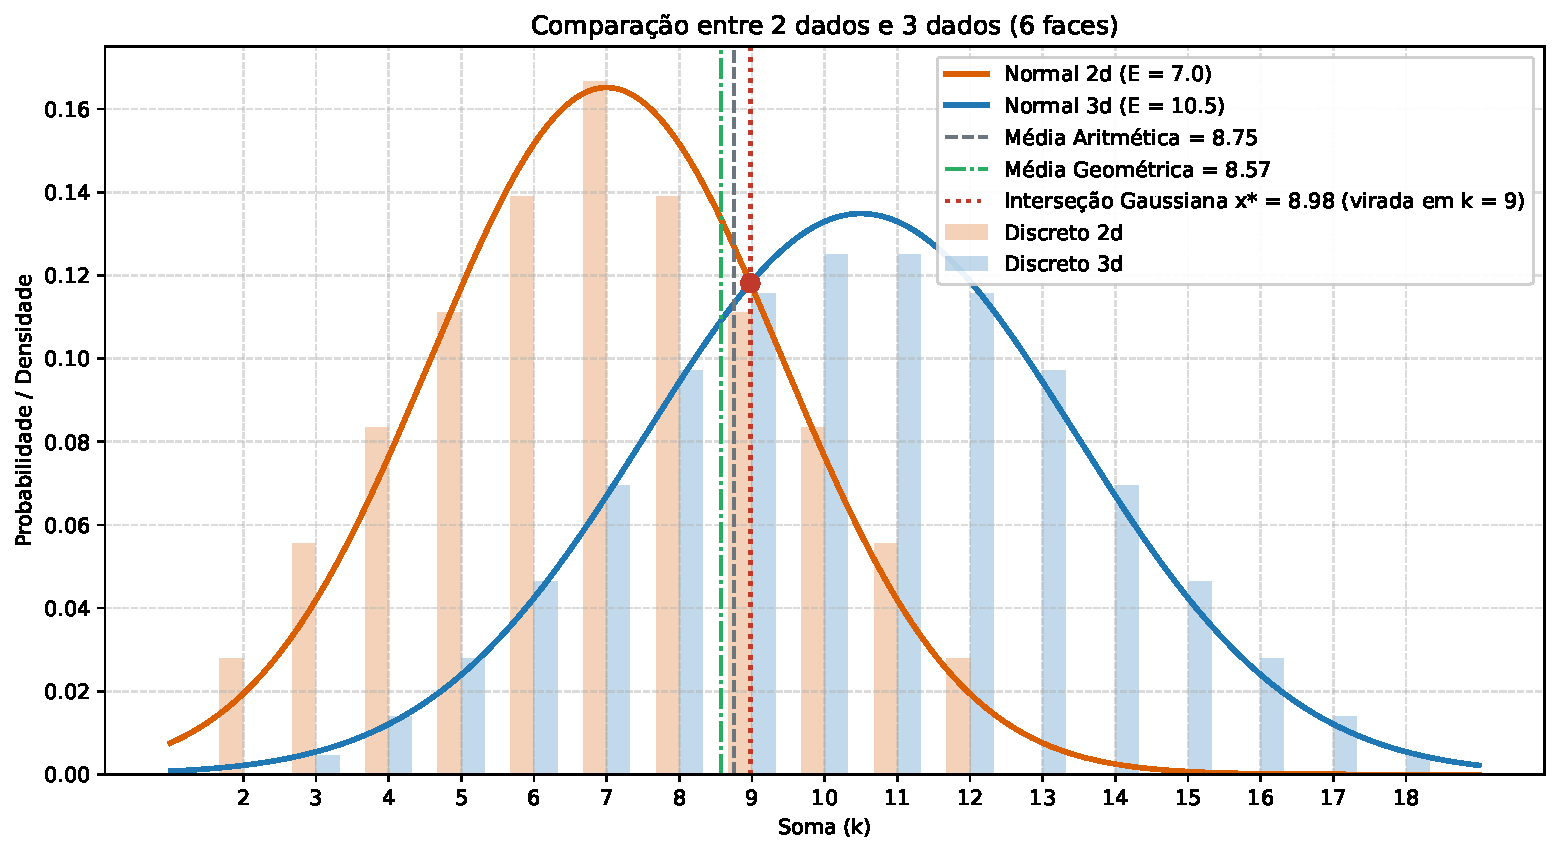
\includegraphics[width=0.88\textwidth]{figures/crossover_2d_3d.pdf}
\caption{Comparação entre $2$ dados e $3$ dados (caso da prova). Como $\mu_A = 8{,}75$ e $x^* \approx 8{,}98$ pertencem ambos ao intervalo $(8, 9)$, a heurística da distância até a média produz a mesma decisão inteira que a distribuição exata.}
\label{fig:crossover_2d_3d}
\end{figure}

\begin{figure}[H]
\centering
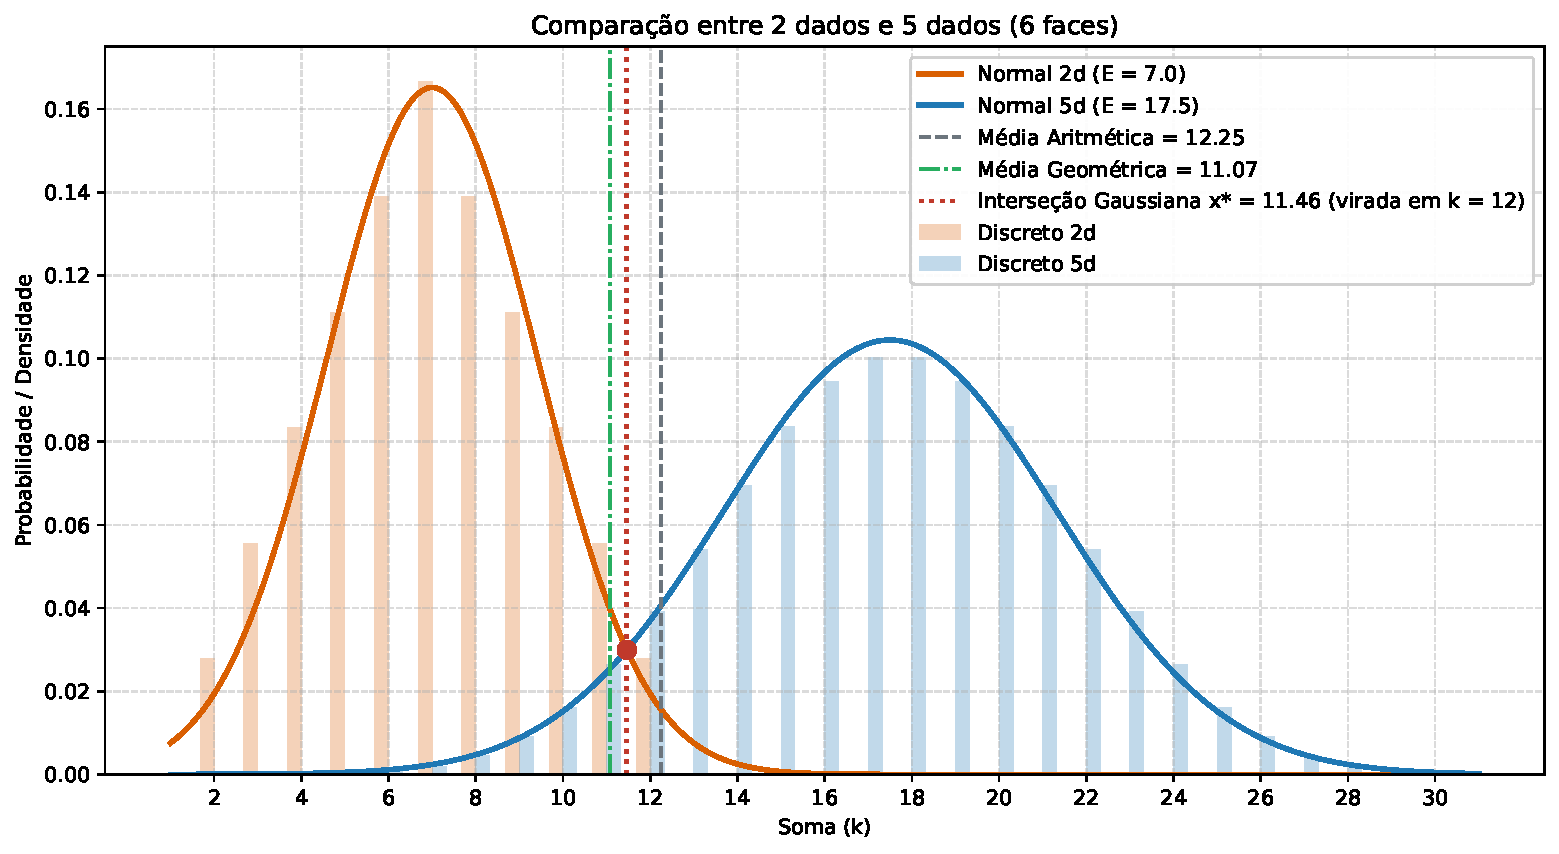
\includegraphics[width=0.88\textwidth]{figures/crossover_2d_5d.pdf}
\caption{Comparação entre $2$ dados e $5$ dados. O ponto de interseção gaussiano $x^* \approx 11{,}46$ ocorre antes do inteiro $k = 12$, enquanto a média aritmética está em $\mu_A = 12{,}25$. Em $k = 12$, $5$ dados já são mais prováveis que $2$ dados ($3{,}92\%$ contra $2{,}78\%$).}
\label{fig:crossover_2d_5d}
\end{figure}

\begin{figure}[H]
\centering
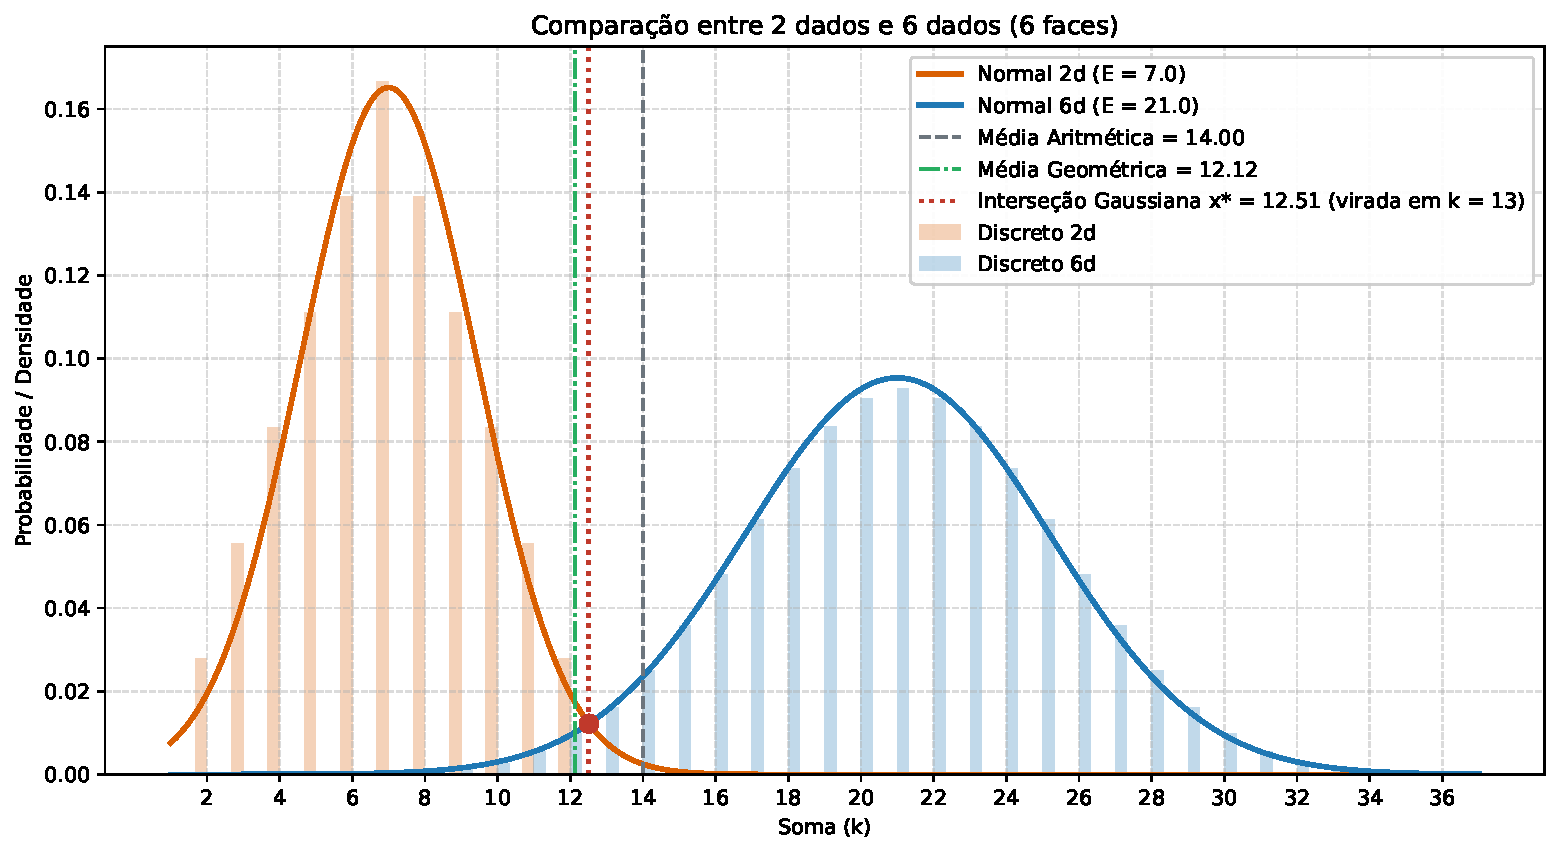
\includegraphics[width=0.88\textwidth]{figures/crossover_2d_6d.pdf}
\caption{Comparação entre $2$ dados e $6$ dados. A média aritmética $\mu_A = 14{,}00$ situa-se fora do suporte de $2$ dados ($k \le 12$), ao passo que a fórmula baseada na média geométrica e logarítmica posiciona a interseção em $x^* \approx 12{,}51$, prevendo corretamente a virada em $k = 13$.}
\label{fig:crossover_2d_6d}
\end{figure}

\section{Conclusão}

A questão da avaliação de Matemática Discreta sobre a probabilidade de obter soma $8$ ou soma $9$ com dois ou três dados ilustra como uma intuição simples pode acertar a resposta final por uma coincidência de arredondamento inteiro. Ao investigarmos por que o critério da distância até a média funcionou naquele caso particular e onde ele falha, demonstramos que:
\begin{enumerate}[topsep=0.2em, itemsep=0.15em]
    \item A heurística da distância até a média equivale a adotar a média aritmética $\mu_A(n,m)$ como fronteira de decisão, desconsiderando que a variância cresce linearmente com o número de dados e que o pico da distribuição decai com $1/\sqrt{n}$.
    \item Para somas de variáveis aleatórias i.i.d., a invariância da razão $\mu_n / \sigma_n^2 = \mu_1 / \sigma_1^2$ anula o termo linear na equação de log-verossimilhança normal, produzindo a expressão fechada $x^*(n,m) = \mu_G(n,m)\sqrt{1 + \mathrm{CV}_1^2 / L(n,m)}$, que une a média geométrica e a média logarítmica.
    \item A comparação entre $x^*(n,m)$ e $\mu_A(n,m)$ divide os pares $(n,m)$ em dois regimes separados pela condição $\mathrm{CV}_1^2 \lessgtr \frac{(m-n)^3}{4nm\ln(m/n)}$: um regime dominado pela altura do pico ($x^* > \mu_A$, gerando contraexemplos como $4\text{d}$ vs $5\text{d}$ na soma $16$) e um regime dominado pela variância ($x^* < \mu_A$, gerando contraexemplos dentro do suporte como $2\text{d}$ vs $5\text{d}$ na soma $12$ e fora do suporte como $2\text{d}$ vs $6\text{d}$ na soma $13$).
\end{enumerate}

Todo o código-fonte desenvolvido em Python para o cálculo combinatório exato, simulação de Monte Carlo e geração das figuras encontra-se disponível publicamente no repositório que acompanha este trabalho.

\section*{Agradecimentos}

O autor agradece ao Prof.\ Dr.\ Jeroen van de Graaf (DCC/ICEx/UFMG) pela receptividade à discussão que deu origem a esta investigação na disciplina de Matemática Discreta, e aos colegas de turma cujas soluções alternativas em prova motivaram a formulação matemática aqui apresentada.

\bibliographystyle{plain}
\bibliography{referencias}

\end{document}
